\chapter{Using \LaTeX}\label{ch:usingLatex}

By reading this chapter and comparing the generated output to the \latex code, one should be able to produce all the necessary content expected of a typeset report. Instructions regarding software installation and compilation are to be found towards the end of the chapter. As with any source code, one should first compile, it to ensure it works. This document should compile with no errors if all the necessary packages are installed. A few warning messages relating to ``Font style'' (Arial) can be ignored. 

\section{Structure of this Template}

The file thesis.tex in the root of the directory (ThesisTemplate) is the main file of this template. This is the file that must be compiled to create the document. The thesis.tex document contains a lot of configuration settings. The only elements that require editing are details such as the title of the report, authors name and so forth. The only further addition to the file is to use the \emph{\textbackslash include} statement to include additional chapters in the report. One may also comment out the \emph{\textbackslash include} statements using the percentage sign (\%) to develop the report on a chapter by chapter basis. The BibTeX database thesis.bib is also included within the root. All the actual content of the report is divided up into directories each with a .tex file containing the chapter content (Appendix~\ref{fig:append:TemplateStructure}).



\section{Using Figures}

 One can insert graphic elements using \latex in a number of ways. Vector based imagery such as diagrams saved to the pdf format may use the \emph{\textbackslash includegraphics} command with the optional \emph{viewport} attribute to specify a precise area of the graphic to be included. Figures should also include a Caption and a Label for referencing.

When inserting a Figure (Figure~\ref{fig:using:VectorGraphicElementPDF}) one uses the \emph{\textbackslash begin\{figure\}} and \emph{\textbackslash end\{figure\}} commands. The image presented is a vector graphic in the form of a pdf file. When working with such files it is usually necessary to include the optional \emph{viewport} attribute to designate the specific area in which to focus. The first pair of coordinates (x~\&~y) designate the pixel location of the lower left corner. The second pair identify the upper right hand corner. Modification of these coordinates allows one to focus in upon a particular area of interest within the vector image. The optional attribute [H] when beginning a Figure inserts the graphic element at the specified location. Other options such as [htb] (here, top, bottom) will place the graphic in the most suitable place that \latex can find. This however can have a negative impact on memory allocation if a large number of images exist.


\begin{figure}[H]
\centering
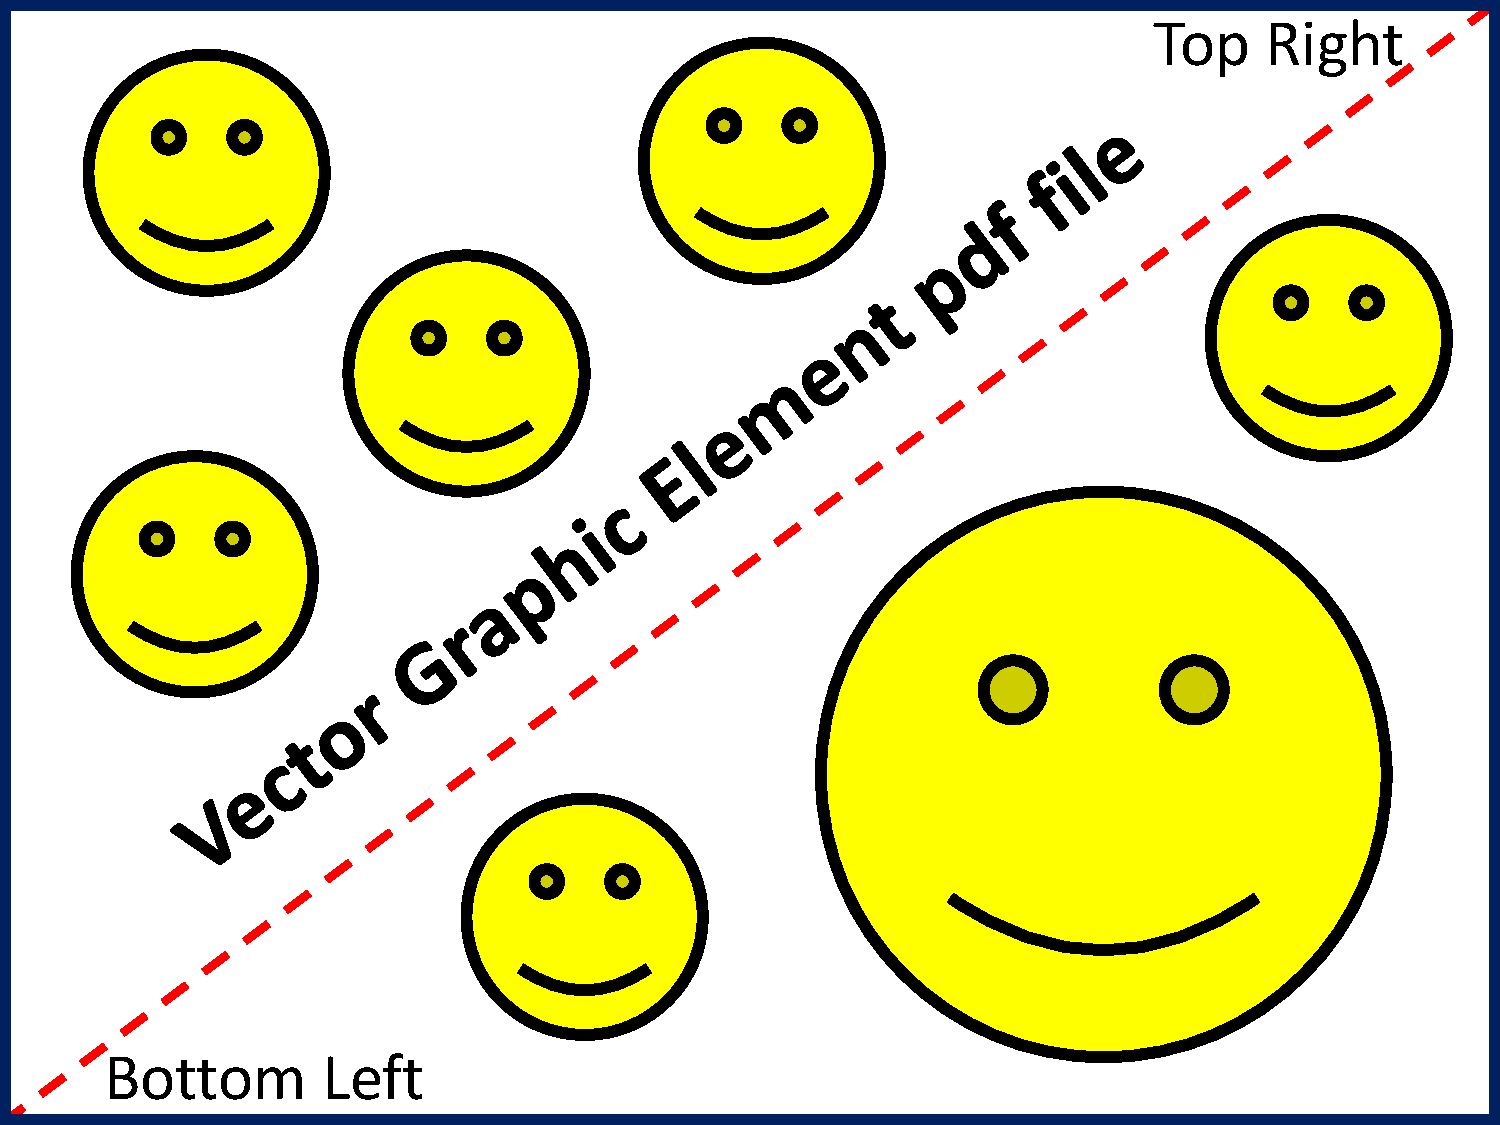
\includegraphics[width=.4\linewidth]{resources/VectorGraphicElementPDF.pdf}
\caption{Vector Graphic - pdf of a PowerPoint Slide}
\label{fig:using:VectorGraphicElementPDF}
\end{figure}

One may use the \emph{minipage} command when inserting two figures to span across the page. This allows for the subdividing of the page into a number of columns of specified width. Figure~\ref{fig:using:Example1} \&~\ref{fig:using:Example2} demonstrate how one may zoom in / focus on a particular section of a graphic by altering the coordinates of the \emph{viewport}. 

\begin{figure}[H]
\begin{minipage}[t]{7.4cm}
\begin{center}
\includegraphics*[viewport= 20 20 600 440, width=.8\linewidth]{resources/VectorGraphicElementPDF.pdf}
\caption{viewport = 20 20 600 440}
\label{fig:using:Example1}
\end{center}
\end{minipage}
\hfill
\begin{minipage}[t]{7.4cm}
\begin{center}
\includegraphics*[viewport= 220 200 400 330, width=.8\linewidth]{resources/VectorGraphicElementPDF.pdf}
\caption{viewport = 220 200 400 330}
\label{fig:using:Example2}
\end{center}
\end{minipage}
\end{figure}

The example below (Figure~\ref{fig:using:samplepngImage}) features a bitmap image. One can see that the extension for the image file isn't specified, as this template is setup to automatically search for .jpg, .png, .gif and .pdf images. The size of the displayed image within the document can be varied by adjusting the height and width attributes. To rotate an image 90 degrees an optional attribute can be added, for example [width=.4\textbackslash linewidth, angle=90].

\begin{figure}[H]
\begin{center}
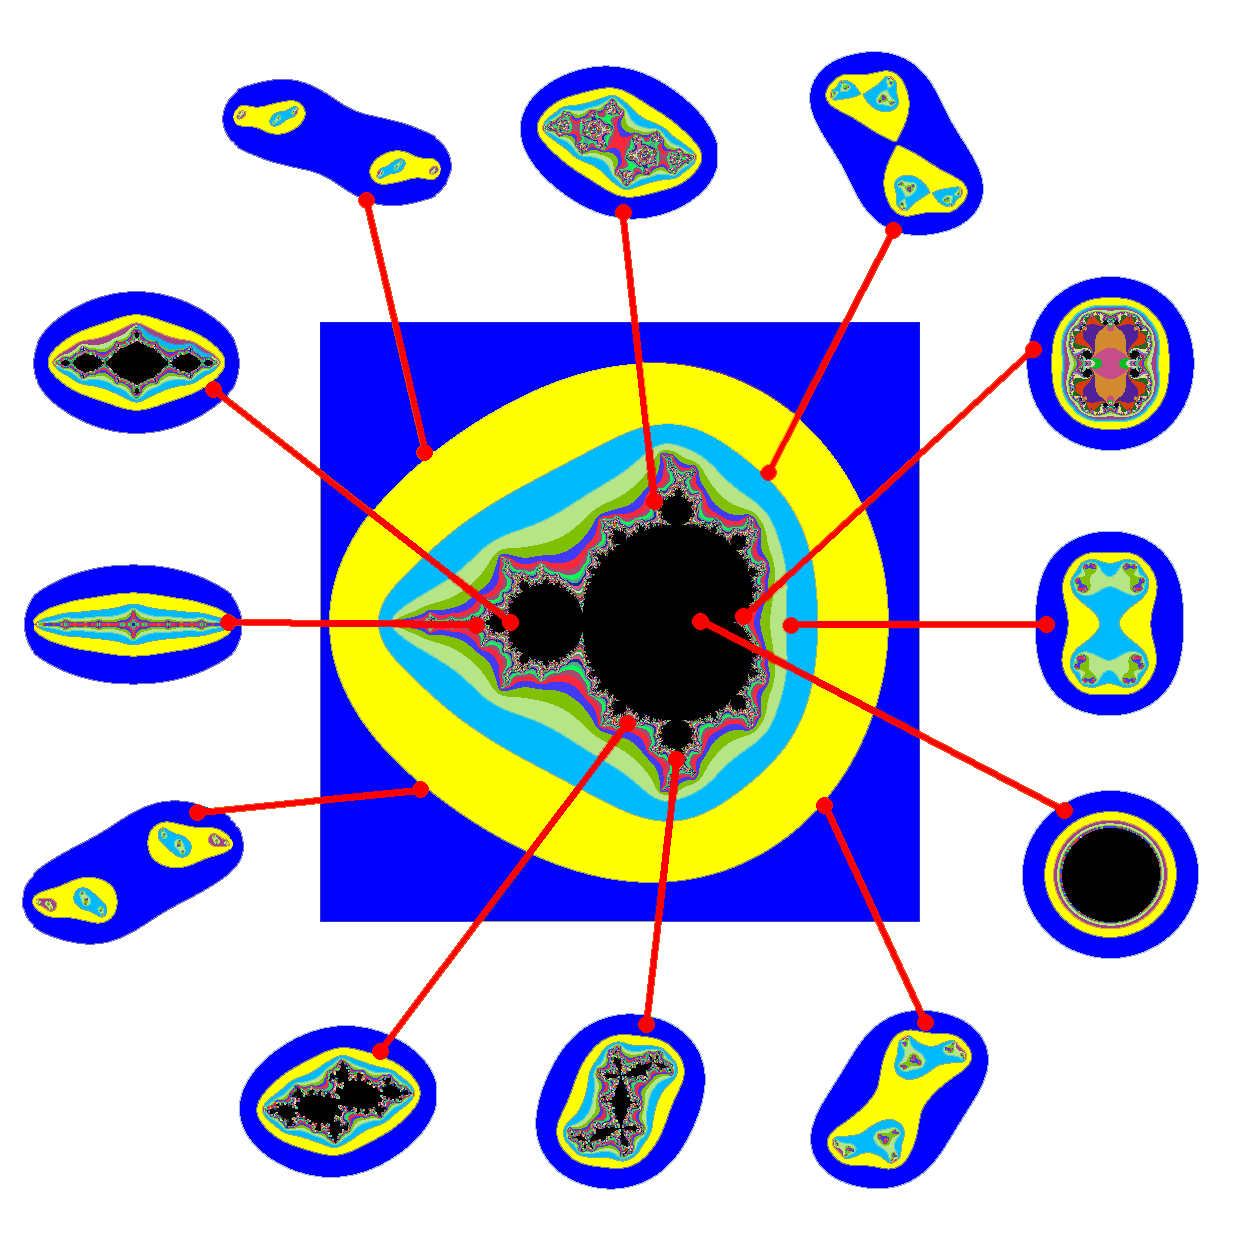
\includegraphics[width=.34\linewidth]{resources/samplepng}
\caption{Caption for Bitmap Image Example} \label{fig:using:samplepngImage}
\end{center}
\end{figure}

\section{Referencing}

To refer to another part of the document one must use a combination of the \emph{\textbackslash ref} and \emph{\textbackslash label} commands. The label is a unique identifier, therefore when working with large documents it helps to give references meaningful names. Examples of this includes prefixing Table references with \emph{tab:}, figures with \emph{fig:}, chapters with \emph{ch:}. In very large documents in may also be useful to add an additional level of prefixing to represent the chapter the label is in. In this example chapter the tables and figures have the additional prefix of \emph{using} to represent the \emph{usingLatex} chapter. The tilde ($\sim$) is used to ensure that a reference remains as a single object. All instances of \emph{\textbackslash ref} should be preceded with the tilde.

\section{Citing Bibliographic References}

Bibliographic references are stored in a database (.bib file extension), this contains a list of articles, proceedings, books, thesis and so forth. Each type of publication has a number of required fields such as a unique identifier, author and title. To cite a reference within the main body text one must use the \emph{\textbackslash cite} and \emph{\textbackslash citep} commands as in the following examples. \cite{book:knuth_1973} for example is well known for his work on the Art of Computer Programming. The SETI@Home project \citep{online:berkeleyBOINC} is an example of a webpage citation. One can also work with articles \citep{art:Russell:1978:Cray1}, MSc Thesis \citep{msc:Shannon:1940}, PhD Thesis \citep{phd:Sutherland:1963} or articles within conference proceedings \citep{proc:Ewald:1978:HPG}. Several other types of published work exist, but they are used to a lesser degree, see the Bath University Library Style guide \citep{online:Bath:2016:HarvardBathStyle}.

\subsection{Compiling a BibTeX Database}

Having initially compiled the document using pdfLatex a number of helper files are created that aid in referencing and citations. One must the compile the bibtex database, followed by an additional two compiles using pdfLatex. Citing additional bibliographic references within the body of the document being produced will require the recompile of the bibtex database. In the case that the bibtex reference of a cited article cannot be found one will see a question mark (?) instead of the proper citation and a compile warning.

\subsection{The Harvard Bibliography Style}

The bibliographic references are laid out using the Harvard referencing style. This style is generally more applicable to humanities rather than the sciences. One would typically expect to see the use of a numbered reference style in the sciences - such as IEEE or Vancouver. In \latex the Harvard style is depreciated. As such alternative solutions are to use the \emph{natbib} or \emph{biblatex} packages, these however yield references of an author, name format, but don't quite conform to a Harvard style. 

Fortunately a Harvard style has been developed at the University of Bath \citep{online:Bath:2016:HarvardBathStyle}. It has been included in this template in the form of a file called \emph{bath.bst}, dated 24 October 2016. The style file can be downloaded as a zip file from the University of Bath Library webpage dedicated to referencing and plagiarism. The zip file includes very useful package documentation, with numerous bibtex examples alongside the resultant output.  

\section{Inserting an Algorithm}

The \emph{algorithm2e} environment \citep{online:Fiorio2016algorithm2e} may be used to generate algorithms (Algorithm~\ref{alg:using:SampleAlgorithm}). If no algorithms are used within the document then comment out \emph{\textbackslash listofalgorithms } in the file {\tt thesis.tex} to remove the list of algorithms page.

\begin{algorithm}
%\dontprintsemicolon
\While{(RANK $<$ COMPSIZE)}{
    \If{(RANK == MASTER)}{
        generate random value \;
        \For{(each item K)}{
            get result \;
        }
    }
}
\caption{A Sample Algorithm} \label{alg:using:SampleAlgorithm}
\end{algorithm}


\section{Table Creation}

The data in Table~\ref{tab:using:TableExample} displays three columns of left-aligned and one column of justified data. The cell contents can be aligned to the left (l), right (r), center (c) or (p). Vertical bars may sometimes be seen in tables but these generally look unprofessional. The Booktabs package \citep{online:Fear2016BookTabs} allows for the creation of professional looking tables as shown in the example.  The use of \emph{\textbackslash toprule}, \emph{\textbackslash midrule} and \emph{\textbackslash bottomrule} commands provided by the package allow for rules of varying thickness and spacing. Data elements (cells / columns) within a table are divided up using the ampersand (\&). To complete a row one must end with a double backslash (\textbackslash\textbackslash). Tables as with figures need a caption and a label. The WinShell editor has a GUI based utility to aid in the creation of the tabular data.

\begin{table}[H]
\caption{Table Caption}\label{tab:using:TableExample}
\centering
\small
\begin{tabular}{lllp{5cm}}
\toprule \textbf{Heading 1}& \textbf{Heading 2}&\textbf{Heading 3}&\textbf{Heading 4}\\
\midrule
Cell A1 & Cell B2 & Cell C3 & Cell D4\\
Cell E1 & Cell F2 & Cell G3 & Justified text with a defined column size of 5cm\\
\bottomrule
\end{tabular}
\end{table}





\section{Inserting Program Code Samples}

To insert small segments of program code (Listing~\ref{code:SampleCode}) that detail how interesting algorithms and so forth are implemented use the \emph{lstlisting} command. Inclusion of program code again requires a Caption and Label. Sample code from external files may also be included (Listing~\ref{code:externalSampleCodeLabel}), by supplying the relative path to the source file. 

\begin{lstlisting}[caption=Sample Program Code Listing, label=code:SampleCode]
if(rndVal==0){
    if(opType > 2){
       //do something
    }
}
\end{lstlisting}

\lstinputlisting[caption={The Caption for the Code Listing},label={code:externalSampleCodeLabel}]{resources/myCodeFile.java}


\section{Working with Maths}
The power of \latex in typesetting mathematical formula is one of its key strengths. The mathematical definition of the ``Cantor set'' is a good example of this in action encompassed within an \emph{\textbackslash equation} environment.

\begin{equation}
\displaystyle\sum_{n=0}^\infty \frac{2^n}{3^{n+1}} = \frac{1}{3} +
\frac{2}{9} + \frac{4}{27} + \frac{8}{81} + \cdots =
\frac{1}{3}\left(\frac{1}{1-\frac{2}{3}}\right) = 1
\end{equation}
 The previous equation demonstrates the use of sigma, fractions, large brackets, power, and dots. The function that defines the MSet $Z_{n+1} =
Z_{n}^2 + C$ is a simpler example of math in use within the body text of a paragraph. Matrix Multiplication is typically regarded as an $O(n^3)$
operation. One may use the \emph{equation} environment for more complex mathematical formula that should standout. For example the product  $C$ of two matrices $A \in M_{n,m}(R)$ and $B \in
M_{m,p}(R)$ may be defined as

\begin{equation}
(A \times B)_{ij} = \sum_{k=0} ^{m-1} a_{ik}b_{kj},~
i=0,...,n-1,~j=0,...,p-1.
\end{equation}

The sizes of the matrices must satisfy $(n \times m)(m \times p) =
(n \times p)$. Matrix multiplication is an associative process
thereby $a\cdot(b \cdot c) = (a \cdot b) \cdot c$. Essentially to
find the value of a particular cell $C_{i,j}$ it is necessary to
multiply row $i$ of the matrix $A$ with column $j$ of matrix $B$
summing all the multiplications.

\section{Using the Correct Quotes}
To surround a piece of text with double quotes one must place two single quotes on either side of the text. The double quote on the left is created using two left quotes (\lq) this is located just above the \emph{tab} key on the keyboard. The right hand double quote is created using two right hand quotes via (\rq) located just above and to the left of the right shift key. A properly formatted quotation should look like ``This is a quotation''. Notice how the direction of the quotes are opposite to one another. A larger example using the \emph{\textbackslash Huge} font size option, is presented below so the quotes can be clearly seen.

\begin{center}
\Huge{``This is a quotation''}
\end{center}


\section{Start Compiling and Editing}
\begin{enumerate}
\item Read the instructions in this file thesisTemplate.pdf, compare the code in the file usingLatex.tex to that of the resultant output of the Using \latex chapter. 

\item Download and install the necessary software - back-end \latex system and front-end text editor. 

\item Compile the files thesis.tex and thesis.bib to generate the file thesis.pdf so that it is identical to file thesisTemplate.pdf.
\begin{enumerate}
\item To achieve this compile with pdfLaTeX, then run BibTeX and compile with pdfLaTeX two further times.

\item It is only necessary to run BibTeX when new citations are added in the thesis document.

\item Two compiles of pdfLaTeX is sufficient to allow for correct references to be established.

\item If one is simply adding additional content (text / figures / tables) then a single compile of pdfLaTeX is sufficient for testing purposes.
\end{enumerate}
\item Note that quite a number of additional files may now be seen in the root and subfolders of the (ThesisTemplate) directory.

\item With a successful compile achieved, start reading through the \latex documents (.tex) to see how the various elements are assembled.

\item Begin editing the document starting with thesis.tex by entering elements such as Thesis Title and Author.

\item When it is necessary to start inserting figures / tables and so forth, copy and paste the \latex code provided and edit as necessary.
\end{enumerate}

\subsection{Required Software}
The implementation of \latex typically used is MikTeX (\url{http://miktex.org}). It is typically best to install the complete MiKTeX  system. A complete system comprises of around 40K files. A minimal install will necessitate the installation of packages as needed. One can individually download and integrate packages into a MikTeX system using the Package Manager (Admin) application. Initially a small installer application must be downloaded and executed. This in-turn downloads the most recent implementation of the MikTeX system. Run the installer again and select the directory of the downloaded package. The MacTeX distribution (\url{http://www.tug.org/mactex/}) is a useful alternative for Mac users. 

The other necessary element is an editor. TeXnicCenter is a free download available at (\url{http://sourceforge.net/projects/texniccenter/}). An alternative is WinEdt a shareware ASCII editor (\url{http://www.winedt.com}). WinEdt can be freely used for a 30 day period, after which one will periodically receive reminders to register the product. Another option for Windows users is WinShell (\url{http://www.winshell.de}). An advantage of WinShell is its in-built BibTeX GUI editor. It also features a useful Table Wizard. For Mac users TexShop (\url{http://pages.uoregon.edu/koch/texshop/}) is a popular option, providing a very easy to use editor. Note the website links in this section were created using the \emph{\textbackslash url} command and included for ease of reference. One should ideally include such references in the Bibliography.  

\section{Conclusion}
Having read this chapter and compared the .tex source to the generated output, one should have all the knowledge necessary to typeset a well formatted and elegant project report. One needs to become familiar with a number of commands, but once mastered it should greatly speedup the report writing process. By using \latex to typeset a document one is removed from a myriad of issues in relation to formatting allowing one to concentrate on the most important task, that of content creation. 
